\chapter{Operational Information}

To classify the picture as closely as possible to the desired result, it was necessary to review the details of the image for any features that could be extracted at an elementary level. The support vector machine implementation in Matlab allowed for as many classification parameters to be passed for generating the classification structure.


\begin{figure}[h]
    \centering
    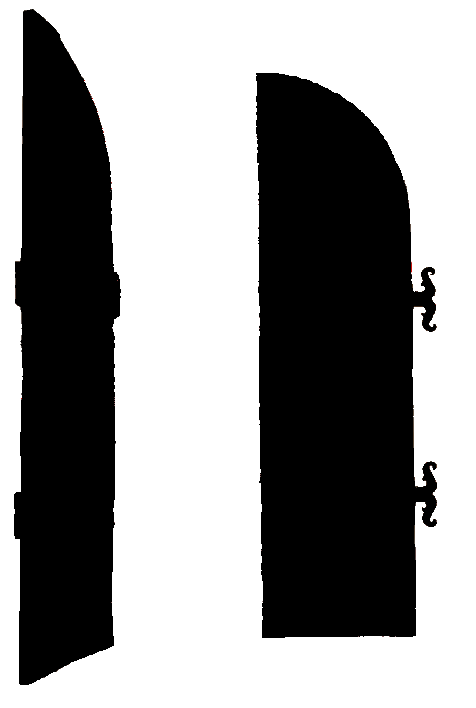
\includegraphics[height=3in]{00_classmask}
    \caption{Classification Mask used to determine class of training points}
    \label{fig:00_classmask}
\end{figure}

When using the class mask, as seen in \ref{fig:00_classmask}, it was necessary to generate a set of points to apply to the mask which maximized the positive effect on the support vector machine while reducing the requirement for an overly high number of required points. 

As explained by Dr. Haykin, the support vector machine internally tries to maximize the distance between the points it is currently training against and the desired hyperplane. \citep{00_SimonHaykin} Randomly generating points from the entire images with no concern for position doesn't benefit the areas in the image where the distinction between both classes is quite complex.

\begin{figure}[h]
    \centering
    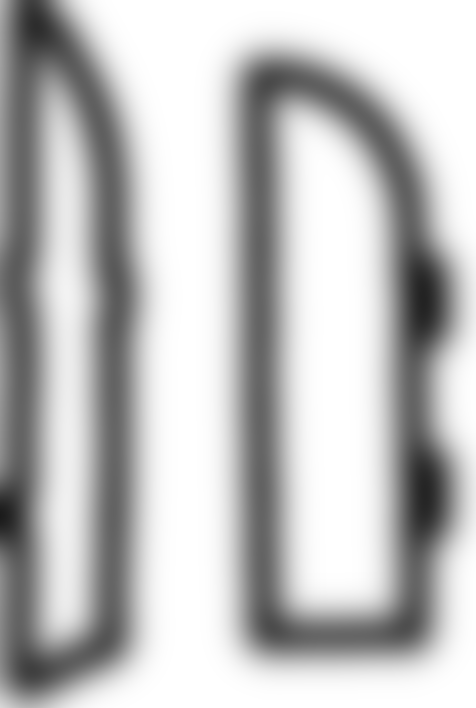
\includegraphics[height=3in]{01_densitymask}
    \caption{Mask relating desired point density to position}
    \label{fig:01_densitymask}
\end{figure}


